\section{累次积分}
\label{sec:integral-iterated}

矩形的面积等于两条边长之积；求一块区域上的总量时，我们也习惯先沿每条竖线累计，再把各条竖线的结果横向相加。前几节的积分只用到一个测度空间。现在有两个测度空间$(X,\mathcal A,\mu)$与$(Y,\mathcal B,\nu)$，需要回答两个问题：乘积集合$X\times Y$上的“面积”怎样由两侧的测度确定；分别对两个坐标累计，什么时候等于整体累计，两种累计次序又何时相同。本节先建立乘积可测结构和乘积测度，再分别给出非负函数与绝对可积函数的换序定理，最后把它们用于欧氏空间中的多重积分和截面计算。

\subsection{乘积可测结构与乘积测度}
\label{sec:integral-product-measure}

\paragraph{可测矩形与乘积\texorpdfstring{$\sigma$}{sigma}代数}
两侧各取一个可测集$A\in\mathcal A$、$B\in\mathcal B$，乘积$A\times B$是最容易确定大小的集合：它的“面积”理应是$\mu(A)\nu(B)$。但圆盘、三角形这类集合都不是这种形式，乘积空间上的可测集合必须由矩形生成。

\begin{definition}[乘积$\sigma$代数]
\label{def:integral-product-sigma-algebra}
设$(X,\mathcal A)$与$(Y,\mathcal B)$是可测空间。形如$A\times B$（$A\in\mathcal A$，$B\in\mathcal B$）的集合称为\term{可测矩形}（measurable rectangle）。由全部可测矩形生成的$\sigma$代数记为$\mathcal A\otimes\mathcal B$，称为\term{乘积$\sigma$代数}（product sigma-algebra）。
\end{definition}

可测矩形全体对有限交封闭：$(A_1\times B_1)\cap(A_2\times B_2)=(A_1\cap A_2)\times(B_1\cap B_2)$。因此它是一个$\pi$系统，后面可以用第二章的$\pi$--$\lambda$定理（定理~\ref{thm:measure-pi-lambda}）比较两个在矩形上取值相同的测度。图~\ref{fig:integral-product-rectangles}(a)中$A$由两个区间组成，矩形$A\times B$因而是两块；(b)说明四分之一圆盘虽然不是矩形，却可以由互不重叠的小矩形逐层填满，成为可数个矩形之并。

\begin{figure}[!htbp]
\centering
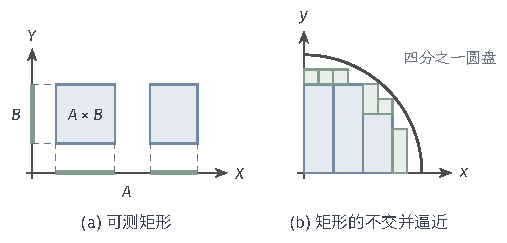
\includegraphics[width=85.93mm]{figures/02-abstract-mathematics/01-metric-and-measure/tikz/c3-product-rectangles/figure.pdf}
\caption{乘积可测结构由矩形生成。(a)取$A=[0.4,1.4]\cup[2.0,2.8]$、$B=[0.5,1.5]$，可测矩形$A\times B$由两块组成，绿色线段分别是$A$与$B$；(b)半径为$2$的四分之一圆盘不是矩形，蓝色矩形按边长$0.5$的网格、绿色矩形按边长$0.25$的网格补充，逐层加细的矩形不交并从内部逼近圆盘。}
\label{fig:integral-product-rectangles}
\end{figure}

\paragraph{截面}
累次积分先固定一个坐标。对$E\subseteq X\times Y$和$x\in X$，称
\[
 E_x=\{y\in Y:(x,y)\in E\}
\]
为$E$在$x$处的\term{截面}（section）；类似地，$E^y=\{x\in X:(x,y)\in E\}$是$E$在$y$处的截面。对函数$f:X\times Y\to\overline{\mathbb R}$，固定$x$得到截面函数$f_x(y)=f(x,y)$，固定$y$得到$f^y(x)=f(x,y)$。图~\ref{fig:integral-sections}中的区域在$x_0$处的截面是一段区间，在$y_0$处的截面却是两段区间：截面的形状取决于固定哪个坐标。

\begin{figure}[!htbp]
\centering
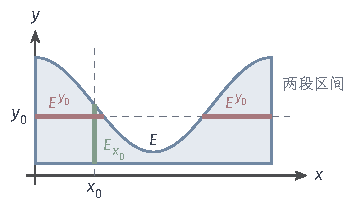
\includegraphics[width=60.187mm]{figures/02-abstract-mathematics/01-metric-and-measure/tikz/c3-sections/figure.pdf}
\caption{同一集合沿两个方向的截面。区域$E=\{(x,y):0\le x\le4,\ 0.2\le y\le1.2+0.8\cos(\pi x/2)\}$；绿色竖线是$x_0=1$处的截面$E_{x_0}=[0.2,1.2]$，红色横线是$y_0=1$处的截面$E^{y_0}$，由$\cos(\pi x/2)\ge-0.25$解得它约为$[0,1.161]\cup[2.839,4]$。}
\label{fig:integral-sections}
\end{figure}

截面运算与集合运算可交换：$(E^{c})_x=(E_x)^{c}$，$(\bigcup_nE_n)_x=\bigcup_n(E_n)_x$。矩形的截面最简单，$(A\times B)_x$在$x\in A$时是$B$，否则是空集。由这两点即可证明乘积可测集的每个截面都可测。

\begin{lemma}[截面可测]
\label{lem:integral-section-measurable}
若$E\in\mathcal A\otimes\mathcal B$，则对每个$x\in X$有$E_x\in\mathcal B$，对每个$y\in Y$有$E^y\in\mathcal A$。若$f$是$\mathcal A\otimes\mathcal B$可测函数，则每个$f_x$是$\mathcal B$可测的，每个$f^y$是$\mathcal A$可测的。
\end{lemma}

\begin{proof}
固定$x$，令$\mathcal C=\{E\in\mathcal A\otimes\mathcal B:E_x\in\mathcal B\}$。上面的两条运算规则说明$\mathcal C$对补集和可数并封闭，且$X\times Y\in\mathcal C$，所以$\mathcal C$是$\sigma$代数；矩形的截面是$B$或空集，故$\mathcal C$包含全部可测矩形，从而包含它们生成的$\mathcal A\otimes\mathcal B$。对函数，任取实数$c$，有$\{y:f_x(y)>c\}=\bigl(\{f>c\}\bigr)_x$，右侧是乘积可测集的截面，属于$\mathcal B$。另一方向的截面同理。
\end{proof}

\paragraph{乘积测度的构造}
对矩形，乘法规则已经给出答案；问题是怎样把它延拓到整个$\mathcal A\otimes\mathcal B$。截面提供了一条直接的途径：把$E$切成截面$E_x$，量出每条截面的大小$\nu(E_x)$，再对$x$累计。为此需要先确认$x\mapsto\nu(E_x)$可测。这里要求两侧测度都$\sigma$有限，即$X$能写成可数个有限测度可测集之并，$Y$也一样（见第~\ref{sec:measure-spaces-def}节）。

\begin{lemma}[截面测度的可测性]
\label{lem:integral-section-measure-measurable}
设$\mu,\nu$都是$\sigma$有限测度，$E\in\mathcal A\otimes\mathcal B$。则$x\mapsto\nu(E_x)$是$X$上取值于$[0,\infty]$的可测函数，$y\mapsto\mu(E^y)$是$Y$上的可测函数。
\end{lemma}

\begin{proof}
先设$\nu(Y)<\infty$。令$\mathcal D$为使$x\mapsto\nu(E_x)$可测的$E\in\mathcal A\otimes\mathcal B$全体。对矩形，$\nu((A\times B)_x)=\nu(B)\mathbf 1_A(x)$可测，所以$\mathcal D$包含可测矩形构成的$\pi$系统。$\mathcal D$是$\lambda$系统：$X\times Y\in\mathcal D$；若$E\in\mathcal D$，则$\nu((E^c)_x)=\nu(Y)-\nu(E_x)$，这里用到$\nu(Y)$有限，差仍可测；若$E_n\in\mathcal D$两两不交，则$\nu((\bigcup_nE_n)_x)=\sum_n\nu((E_n)_x)$是可测函数之和的极限。由$\pi$--$\lambda$定理，$\mathcal D$包含矩形生成的$\sigma$代数，即$\mathcal D=\mathcal A\otimes\mathcal B$。

一般情形取递增的$Y_n\in\mathcal B$，使$\nu(Y_n)<\infty$且$\bigcup_nY_n=Y$。对有限测度$\nu_n(B)=\nu(B\cap Y_n)$应用上一段，$x\mapsto\nu(E_x\cap Y_n)$可测；由测度的从下连续性，它随$n$递增到$\nu(E_x)$，可测函数列的极限仍可测。另一方向对称。
\end{proof}

有了可测性，就可以对截面测度积分。下面的定理同时说明，先切竖线和先切横线得到同一个乘积测度。

\begin{theorem}[乘积测度的存在唯一性]
\label{thm:integral-product-measure-exists}
设$(X,\mathcal A,\mu)$与$(Y,\mathcal B,\nu)$是$\sigma$有限测度空间。在$\mathcal A\otimes\mathcal B$上存在唯一的测度$\pi$，使对所有$A\in\mathcal A$、$B\in\mathcal B$都有
\begin{equation}
 \pi(A\times B)=\mu(A)\nu(B),
 \label{eq:integral-product-rectangle}
\end{equation}
其中约定$0\cdot\infty=0$。并且对每个$E\in\mathcal A\otimes\mathcal B$，
\begin{equation}
 \pi(E)=\int_X\nu(E_x)\,\mathrm d\mu(x)=\int_Y\mu(E^y)\,\mathrm d\nu(y).
 \label{eq:integral-product-sections}
\end{equation}
\end{theorem}

\begin{proof}
令$\pi_1(E)=\int_X\nu(E_x)\,\mathrm d\mu(x)$，由引理~\ref{lem:integral-section-measure-measurable}，被积函数非负可测，定义有意义。$\pi_1(\varnothing)=0$。若$E_n$两两不交，则各截面$(E_n)_x$也两两不交，$\nu((\bigcup_nE_n)_x)=\sum_n\nu((E_n)_x)$；非负函数项级数可以逐项积分（单调收敛定理~\ref{thm:integral-monotone-convergence}用于部分和），故$\pi_1(\bigcup_nE_n)=\sum_n\pi_1(E_n)$，$\pi_1$是测度。对矩形，$\pi_1(A\times B)=\int_X\nu(B)\mathbf 1_A\,\mathrm d\mu=\mu(A)\nu(B)$。同样，$\pi_2(E)=\int_Y\mu(E^y)\,\mathrm d\nu(y)$也是满足式~\eqref{eq:integral-product-rectangle}的测度。

唯一性：取$X_n\in\mathcal A$、$Y_m\in\mathcal B$分别覆盖$X$、$Y$且测度有限，则可数个矩形$X_n\times Y_m$覆盖$X\times Y$，每个在任何满足式~\eqref{eq:integral-product-rectangle}的测度下都有有限值。两个这样的测度在生成$\pi$系统上相等，又被该$\pi$系统中一列有限测度集合覆盖，由第二章的唯一性结论（定理~\ref{thm:measure-pi-lambda}）在$\mathcal A\otimes\mathcal B$上相等。特别地$\pi_1=\pi_2$，这正是式~\eqref{eq:integral-product-sections}。
\end{proof}

\begin{definition}[乘积测度]
\label{def:integral-product-measure}
定理~\ref{thm:integral-product-measure-exists}中的唯一测度称为$\mu$与$\nu$的\term{乘积测度}（product measure），记为$\mu\otimes\nu$；测度空间$(X\times Y,\mathcal A\otimes\mathcal B,\mu\otimes\nu)$称为两者的乘积测度空间。
\end{definition}

矩形规则~\eqref{eq:integral-product-rectangle}只在矩形上指定数值，不是对所有集合的定义；把它延拓到$\mathcal A\otimes\mathcal B$并保证唯一，靠的是截面积分构造和$\pi$--$\lambda$唯一性。也可以先用矩形规则定义外测度，再走第二章的Carathéodory延拓（定理~\ref{thm:measure-caratheodory}），得到的是同一个测度。

\begin{example}[有限网格上的乘积测度]
\label{ex:integral-finite-product}
取$X=\{1,2\}$，$\mu(\{1\})=1$、$\mu(\{2\})=2$；$Y=\{a,b,c\}$，$\nu(\{a\})=1$、$\nu(\{b\})=3$、$\nu(\{c\})=1$。乘积测度给单点$(i,y)$的质量$\mu(\{i\})\nu(\{y\})$，六个格点的质量依次为$1,3,1,2,6,2$。取$E=\{(1,a),(1,b),(2,b),(2,c)\}$，按竖线累计，$\nu(E_1)=4$、$\nu(E_2)=4$，$(\mu\otimes\nu)(E)=1\cdot4+2\cdot4=12$；按横线累计，$\mu(E^a)=1$、$\mu(E^b)=3$、$\mu(E^c)=2$，结果为$1\cdot1+3\cdot3+2\cdot1=12$。两种切法得到同一个数，正是式~\eqref{eq:integral-product-sections}。
\end{example}

\paragraph{完备化与截面}
乘积测度空间一般不完备。第二章已经指出，$\mathbb R$中存在不Lebesgue可测的子集（第~\ref{sec:measure-construction}节）。取一个这样的集合$N\subseteq\mathbb R$，集合$\{0\}\times N$包含在$\{0\}\times\mathbb R$之中，后者是矩形，$(\lambda\otimes\lambda)$测度为$0\cdot\infty=0$。所以$\{0\}\times N$属于$\lambda\otimes\lambda$的完备化，但它在$x=0$处的截面$N$不可测。

可见完备化以后，引理~\ref{lem:integral-section-measurable}不能保持为“每个截面都可测”。不过坏截面只出现在零测的$x$上，下面的Fubini定理会给出相应的“几乎每个截面”版本。使用完备化的乘积测度时，截面性质都应当理解为在一个零测例外集之外成立。

\subsection{Tonelli定理}
\label{sec:integral-tonelli}

式~\eqref{eq:integral-product-sections}说的是示性函数$\mathbf 1_E$的整体积分等于两种次序的累次积分。对一般非负函数，沿积分的构造步骤把这一结论推广过去：示性函数、简单函数、递增极限。非负贡献不会相互抵消，所以结论允许各方都等于$+\infty$。先对一个变量积分、再对另一个变量积分所得的量称为\term{累次积分}（iterated integral）。

\begin{theorem}[Tonelli定理]
\label{thm:analysis-tonelli-fubini}
设$(X,\mathcal A,\mu)$与$(Y,\mathcal B,\nu)$是$\sigma$有限测度空间，$f:X\times Y\to[0,\infty]$是$\mathcal A\otimes\mathcal B$可测函数。则
\[
 x\longmapsto\int_Yf(x,y)\,\mathrm d\nu(y),\qquad y\longmapsto\int_Xf(x,y)\,\mathrm d\mu(x)
\]
分别是$X$与$Y$上的可测函数，并且
\begin{equation}
 \begin{aligned}
 \int_{X\times Y}f\,\mathrm d(\mu\otimes\nu)
 &=\int_X\Bigl(\int_Yf(x,y)\,\mathrm d\nu(y)\Bigr)\mathrm d\mu(x)\\
 &=\int_Y\Bigl(\int_Xf(x,y)\,\mathrm d\mu(x)\Bigr)\mathrm d\nu(y),
 \end{aligned}
 \label{eq:integral-tonelli}
\end{equation}
三者可以同为$+\infty$。
\end{theorem}

\begin{proof}
由引理~\ref{lem:integral-section-measurable}，各截面可测，内层积分有意义。证明按函数的构造分四步。

第一步，$f$是矩形$A\times B$的示性函数。内层积分是$\nu(B)\mathbf 1_A(x)$，外层得$\mu(A)\nu(B)$，与整体积分$(\mu\otimes\nu)(A\times B)$相同。第二步，$f=\mathbf 1_E$，$E\in\mathcal A\otimes\mathcal B$。内层积分是$\nu(E_x)$，其可测性来自引理~\ref{lem:integral-section-measure-measurable}，而它的积分等于$(\mu\otimes\nu)(E)$正是式~\eqref{eq:integral-product-sections}；第一步到第二步的推广由该引理中的$\pi$--$\lambda$论证完成。

第三步，$f=\sum_{i=1}^mc_i\mathbf 1_{E_i}$是非负简单函数。内层积分是$\sum_ic_i\nu((E_i)_x)$，仍可测；由非负积分的线性性，三项都等于$\sum_ic_i(\mu\otimes\nu)(E_i)$。

第四步，一般非负可测$f$。由引理~\ref{lem:integral-simple-approx}取非负简单函数列$s_n\uparrow f$。对每个$x$，截面$(s_n)_x\uparrow f_x$，单调收敛定理给出$\int_Ys_n(x,y)\,\mathrm d\nu(y)\uparrow\int_Yf(x,y)\,\mathrm d\nu(y)$；可测函数的递增极限可测，所以内层积分函数可测。再对外层和整体积分各用一次单调收敛，第三步的等式在极限中保持。另一种次序同理。
\end{proof}

\term{Tonelli定理}也给出一个实用的判断：要检查乘积空间上的非负函数是否可积，只需任选一种方便的次序计算累次积分。

\paragraph{$\sigma$有限条件}
定理中的$\sigma$有限条件不能省去。取$X=Y=[0,1]$，$\mu=\lambda$为Lebesgue测度，$\nu$为$[0,1]$的Borel集上的计数测度；后者不$\sigma$有限，因为可数个有限集之并仍可数。令$I_{n,k}=[(k-1)/n,k/n]$，对角线
\[
 D=\{(x,x):x\in[0,1]\}=\bigcap_{n\ge1}\bigcup_{k=1}^n(I_{n,k}\times I_{n,k})
\]
是可测矩形的可数交并，属于乘积$\sigma$代数：右侧的点满足对每个$n$，两坐标落在同一条长$1/n$的区间里，所以两坐标相等。先对$y$累计，$\nu(D_x)=\nu(\{x\})=1$，再对$x$积分得$1$；先对$x$累计，$\lambda(D^y)=\lambda(\{y\})=0$，再积分得$0$。两种次序的结果不同，问题出在计数测度无法被有限质量的集合可数覆盖，定理~\ref{thm:integral-product-measure-exists}的唯一性论证不再可用。

\paragraph{非负双重级数}
当一侧或两侧取计数测度时，Tonelli定理就是非负级数的换序规则。取$X=Y=\mathbb N_{\ge1}$并都配计数测度，它们$\sigma$有限；由第~\ref{sec:integral-classical}节，计数测度的积分就是求和。对$a_{i,j}\ge0$，定理给出
\[
 \sum_{(i,j)}a_{i,j}=\sum_{i=1}^\infty\sum_{j=1}^\infty a_{i,j}=\sum_{j=1}^\infty\sum_{i=1}^\infty a_{i,j},
\]
三者可同为$+\infty$。例如取$a_{i,j}=2^{-i}\mathbf 1\{j\le i\}$。先对$i$求和，$\sum_{i\ge j}2^{-i}=2^{1-j}$，再对$j$求和得$2$；先对$j$求和，第$i$行有$i$个非零项，得$i2^{-i}$。于是$\sum_{i\ge1}i2^{-i}=2$，换序直接算出了这个级数的和。

若一侧取计数测度、另一侧取一般$\sigma$有限测度$\mu$，Tonelli定理变成$\int_X\sum_nf_n\,\mathrm d\mu=\sum_n\int_Xf_n\,\mathrm d\mu$（$f_n\ge0$），这就是第~\ref{sec:integral-limits}节非负函数项级数的逐项积分。两种情形说的是同一件事：非负质量不论按什么次序累计，总量都一样；这里还不需要任何绝对可积性。

\subsection{Fubini定理}
\label{sec:integral-fubini}

被积函数可正可负时，两种次序可能以不同方式抵消正负贡献。处理方法是先用Tonelli定理控制绝对值，确认正负两部分的总量都有限，再分别换序后相减。

\begin{theorem}[Fubini定理]
\label{thm:integral-fubini}
设$(X,\mathcal A,\mu)$与$(Y,\mathcal B,\nu)$是$\sigma$有限测度空间，$f$是$X\times Y$上$\mathcal A\otimes\mathcal B$可测的实值或复值函数，且
\[
 \int_{X\times Y}|f|\,\mathrm d(\mu\otimes\nu)<\infty.
\]
则存在$\mu$零测集$N\in\mathcal A$，使对$x\notin N$，截面$f_x$关于$\nu$可积；令$I(x)=\int_Yf(x,y)\,\mathrm d\nu(y)$（$x\notin N$）、$I(x)=0$（$x\in N$），则$I$关于$\mu$可积，且
\begin{equation}
 \begin{aligned}
 \int_{X\times Y}f\,\mathrm d(\mu\otimes\nu)&=\int_XI\,\mathrm d\mu\\
 &=\int_Y\Bigl(\int_Xf(x,y)\,\mathrm d\mu(x)\Bigr)\mathrm d\nu(y),
 \end{aligned}
 \label{eq:integral-fubini}
\end{equation}
最后一项按同样方式在一个$\nu$零测集之外理解。
\end{theorem}

\begin{proof}
对$|f|$应用Tonelli定理，$J(x)=\int_Y|f(x,y)|\,\mathrm d\nu(y)$是可测函数且$\int_XJ\,\mathrm d\mu<\infty$。可积的非负函数几乎处处有限，故$N=\{J=\infty\}$可测且$\mu(N)=0$；$x\notin N$时$f_x$可积。

先设$f$为实值。正部$f^+$与负部$f^-$都不超过$|f|$，都是非负乘积可测函数。分别对它们应用Tonelli定理：$x\mapsto\int_Yf^\pm(x,y)\,\mathrm d\nu(y)$可测，积分都等于$\int f^\pm\,\mathrm d(\mu\otimes\nu)<\infty$。在$X\setminus N$上两者都有限，$I=\int_Yf_x^+\,\mathrm d\nu-\int_Yf_x^-\,\mathrm d\nu$；在$N$上改值不影响外层积分。由有限积分的线性性，
\[
 \int_XI\,\mathrm d\mu=\int f^+\,\mathrm d(\mu\otimes\nu)-\int f^-\,\mathrm d(\mu\otimes\nu)=\int f\,\mathrm d(\mu\otimes\nu).
\]
复值情形对实部和虚部分别应用实值结论，它们的绝对值都不超过$|f|$。另一种次序同理。
\end{proof}

Tonelli定理与\term{Fubini定理}合起来给出使用顺序：先对$|f|$任选一种次序计算非负累次积分；若结果有限，Fubini定理允许对$f$本身在两种次序之间自由切换。只算出$f$的两个累次积分并不构成检查，下面的两个例子都满足“各自算得出”，却不满足绝对可积。

\paragraph{完备化后的截面}
若$\mu,\nu$本身完备，常用的是$\mu\otimes\nu$的完备化，例如$\mathbb R^2$上的Lebesgue测度。设$f$关于完备化可测。由完备化的定义，示性函数$\mathbf 1_F$总与某个乘积可测示性函数只在一个乘积可测零测集内不同，经简单函数逼近，$f$与某个$\mathcal A\otimes\mathcal B$可测函数$g$也只在一个零测集$M\in\mathcal A\otimes\mathcal B$内不同。对$\mathbf 1_M$用Tonelli定理，$\int_X\nu(M_x)\,\mathrm d\mu=0$，所以几乎每个$x$都有$\nu(M_x)=0$。对这些$x$，$f_x$与$g_x$只在$\nu$零测集上不同，$\nu$完备保证$f_x$可测，并且积分相同。因此Tonelli与Fubini定理对完备化仍成立，只是截面可测、内层积分可测这些结论改为对几乎每个$x$（或$y$）成立。上一小节$\{0\}\times N$的例子说明这个“几乎每个”无法去掉。

\paragraph{缺少绝对可积时的反例}
最直接的反例来自双重级数。取无穷矩阵$a_{i,j}=\mathbf 1\{j=i\}-\mathbf 1\{j=i+1\}$（$i,j\ge1$），即主对角线上为$+1$、紧邻其右的对角线上为$-1$，其余为零，并在$\mathbb N_{\ge1}\times\mathbb N_{\ge1}$上配计数测度。每一行恰有一个$+1$和一个$-1$，行和为$0$；第一列只有$a_{1,1}=1$，第$j\ge2$列有$a_{j,j}=1$与$a_{j-1,j}=-1$，列和分别为$1,0,0,\ldots$。于是
\[
 \sum_{i=1}^\infty\sum_{j=1}^\infty a_{i,j}=0,\qquad
 \sum_{j=1}^\infty\sum_{i=1}^\infty a_{i,j}=1.
\]
图~\ref{fig:integral-fubini-counterexample}显示了配对方式的差别：逐行求和时每个$+1$与同一行右侧的$-1$抵消；逐列求和时每个$-1$与同一列下方的$+1$抵消，第一列的$+1$则找不到配对对象。每行绝对值之和为$2$，所以$\sum_{i,j}|a_{i,j}|=\infty$，Fubini定理的条件不成立。

\begin{figure}[!htbp]
\centering
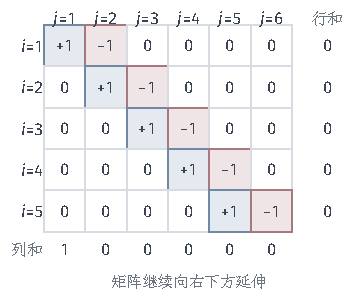
\includegraphics[width=59.951mm]{figures/02-abstract-mathematics/01-metric-and-measure/tikz/c3-fubini-counterexample/figure.pdf}
\caption{无穷矩阵$a_{i,j}=\mathbf 1\{j=i\}-\mathbf 1\{j=i+1\}$的左上角五行六列，矩阵向右下方继续。蓝色单元为$+1$，红色单元为$-1$；每一整行的和为$0$，第一整列的和为$1$，其余整列的和为$0$（第六列的$+1$位于第六行，在图外）。}
\label{fig:integral-fubini-counterexample}
\end{figure}

连续函数也会出现同样的现象。在$(0,1)^2$上取
\[
 f(x,y)=\frac{x^2-y^2}{(x^2+y^2)^2}.
\]
直接求导得$\partial_y\bigl(y/(x^2+y^2)\bigr)=(x^2-y^2)/(x^2+y^2)^2=f(x,y)$，所以固定$x\in(0,1)$时
\[
 \int_0^1f(x,y)\,\mathrm dy=\Bigl[\frac{y}{x^2+y^2}\Bigr]_{y=0}^{y=1}=\frac1{1+x^2},
 \qquad
 \int_0^1\frac{\mathrm dx}{1+x^2}=\frac\pi4.
\]
由于$f(y,x)=-f(x,y)$，先对$x$积分的内层结果是$-1/(1+y^2)$，这一次序得到$-\pi/4$。两种次序的结果都有限却不相等，原因仍是绝对可积性失效。在$0<y<x$处$f>0$，因此
\[
 \int_0^1|f(x,y)|\,\mathrm dy\ge\int_0^xf(x,y)\,\mathrm dy=\Bigl[\frac{y}{x^2+y^2}\Bigr]_{y=0}^{y=x}=\frac1{2x},
\]
而$\int_0^1(2x)^{-1}\,\mathrm dx=\infty$，由Tonelli定理，$\int_{(0,1)^2}|f|\,\mathrm d\lambda_2=\infty$。用极坐标看，$|f|=|\cos2\theta|/r^2$，面积元带一个$r$，原点附近的径向积分$\int_0^1r^{-1}\,\mathrm dr$发散；正、负两部分在原点附近各自累计出无穷，先积哪个变量决定了两者怎样相减。

\subsection{多重积分与截面计算}
\label{sec:integral-multiple}

\paragraph{有限乘积与Lebesgue测度}
三个或更多因子的乘积可以逐次组成。对$\sigma$有限测度空间$(X_k,\mathcal A_k,\mu_k)$（$k=1,2,3$），$(\mathcal A_1\otimes\mathcal A_2)\otimes\mathcal A_3$与$\mathcal A_1\otimes(\mathcal A_2\otimes\mathcal A_3)$都由“三重矩形”$A_1\times A_2\times A_3$生成，因而相同；两种组合方式得到的乘积测度在三重矩形上都等于$\mu_1(A_1)\mu_2(A_2)\mu_3(A_3)$，三重矩形是对有限交封闭且可被有限测度者可数覆盖的生成族，由唯一性它们相同。因此$\mu_1\otimes\cdots\otimes\mu_d$与组合括号无关，反复使用Tonelli或Fubini定理，非负或绝对可积的多重积分可以按任意坐标次序逐次计算。无限多个坐标的乘积以及随机过程分布的构造需要另外的工具，留给概率空间与随机过程的相关部分。

剩下要核对的是，第二章用轴平行矩形直接构造的$d$维Lebesgue测度$\lambda_d$与逐次乘积是否相同（第~\ref{sec:measure-construction}节）。

\begin{theorem}[Lebesgue测度与乘积测度相容]
\label{thm:integral-lebesgue-product}
对$p,q\ge1$，$\mathcal B(\mathbb R^p)\otimes\mathcal B(\mathbb R^q)=\mathcal B(\mathbb R^{p+q})$，并且在这个$\sigma$代数上$\lambda_{p+q}=\lambda_p\otimes\lambda_q$。特别地，$\lambda_d$在Borel集上等于$d$个一维Lebesgue测度的乘积。
\end{theorem}

\begin{proof}
$\mathbb R^{p+q}$中的开集是可数个有理端点开盒之并，每个开盒是$\mathbb R^p$与$\mathbb R^q$中开盒的乘积，属于$\mathcal B(\mathbb R^p)\otimes\mathcal B(\mathbb R^q)$，故右侧的Borel $\sigma$代数包含在左侧。反过来，固定$B\in\mathcal B(\mathbb R^q)$，投影$(\bm x,\bm y)\mapsto\bm x$连续，$A\times\mathbb R^q$是Borel集$A$在连续映射下的原像，因此对Borel集$A$是Borel集；同理$\mathbb R^p\times B$是Borel集，两者之交$A\times B$也是，故左侧包含在右侧。

两测度在形如$\prod_{k=1}^{p+q}(a_k,b_k]$的有界半开盒上都等于各边长之积：在乘积一侧，这样的盒是$\mathbb R^p$与$\mathbb R^q$中两个半开盒的乘积。这些盒对有限交封闭（交集仍是半开盒或空集），生成$\mathcal B(\mathbb R^{p+q})$，并且可数个盒$[-n,n]^{p+q}$覆盖全空间且测度有限。由唯一性定理，两测度在Borel集上相同。
\end{proof}

$\lambda_d$定义在Lebesgue可测集$\mathcal L(\mathbb R^d)$上，它是Borel测度的完备化（第~\ref{sec:measure-construction}节），所以$(\mathbb R^{p+q},\mathcal L(\mathbb R^{p+q}),\lambda_{p+q})$是$\lambda_p\otimes\lambda_q$的完备化。对Lebesgue可测函数使用累次积分时，应采用上一小节的“几乎每个截面”版本。卷一用Riemann和建立了长方体和简单区域上的累次积分，被积函数通常连续，可参考\BookChapterRef{chap:multivariate-integration}{卷一“多元函数积分”章}；在那里成立的计算，在连续函数于有界闭区域上绝对可积的条件下，就是这里Fubini定理的特例，而Tonelli与Fubini定理还覆盖了无界区域、不连续函数和一般测度。

\paragraph{区域积分与切片}
对可测区域$E\subseteq X\times Y$，区域上的积分定义为$\int_Ef\,\mathrm d(\mu\otimes\nu)=\int f\mathbf 1_E\,\mathrm d(\mu\otimes\nu)$。函数$f\mathbf 1_E$的截面在$E_x$之外取零，于是在相应条件下
\[
 \int_Ef\,\mathrm d(\mu\otimes\nu)=\int_X\Bigl(\int_{E_x}f(x,y)\,\mathrm d\nu(y)\Bigr)\mathrm d\mu(x).
\]
内层积分的范围就是截面$E_x$；交换次序时，要按另一个方向重新读出截面$E^y$，而不是只交换微分记号。

\begin{example}[换序计算含$e^{y^2}$的累次积分]
\label{ex:integral-order-swap}
考虑$\int_0^1\bigl(\int_x^1e^{y^2}\,\mathrm dy\bigr)\mathrm dx$。内层的$e^{y^2}$没有初等原函数，按原次序无法直接用原函数计算。积分区域是三角形$E=\{(x,y):0\le x\le y\le1\}$，被积函数非负，Tonelli定理允许换序；$E$在固定$y$处的截面是$E^y=[0,y]$，所以
\[
 \int_0^1\Bigl(\int_0^ye^{y^2}\,\mathrm dx\Bigr)\mathrm dy=\int_0^1ye^{y^2}\,\mathrm dy=\frac{e-1}2.
\]
内层对$x$积分时$e^{y^2}$是常数，只产生截面长度$y$，而这个因子恰好使外层有原函数$\frac12e^{y^2}$。
\end{example}

\paragraph{层饼公式}
截面方法还能把一个积分改写成“按高度分层”的累计。设$(X,\mathcal A,\mu)$$\sigma$有限，$f:X\to[0,\infty]$可测，考察图像下方的区域
\[
 \Gamma=\{(x,t)\in X\times(0,\infty):0<t<f(x)\}.
\]
若$0<t<f(x)$，可以取有理数$r$使$t<r<f(x)$，所以$\Gamma=\bigcup_{r\in\mathbb Q,\,r>0}\bigl(\{f>r\}\times(0,r)\bigr)$，是可数个可测矩形之并，属于$\mathcal A\otimes\mathcal B(\mathbb R)$。对$\mathbf 1_\Gamma$用Tonelli定理计算$(\mu\otimes\lambda)(\Gamma)$的两种次序。

\begin{theorem}[层饼公式]
\label{thm:integral-layer-cake}
设$(X,\mathcal A,\mu)$是$\sigma$有限测度空间，$f:X\to[0,\infty]$可测。则
\begin{equation}
 \int_Xf\,\mathrm d\mu=\int_0^\infty\mu(\{f>t\})\,\mathrm dt,
 \label{eq:integral-layer-cake}
\end{equation}
两侧可以同为$+\infty$。
\end{theorem}

\begin{proof}
固定$x$，$\Gamma_x=(0,f(x))$，长度为$f(x)$（$f(x)=\infty$时为$\infty$），先对$t$累计得$\int_Xf\,\mathrm d\mu$。固定$t>0$，$\Gamma^t=\{x:f(x)>t\}$，先对$x$累计得$\int_0^\infty\mu(\{f>t\})\,\mathrm dt$。两者都等于$(\mu\otimes\lambda)(\Gamma)$。
\end{proof}

这个结果称为\term{层饼公式}（layer cake formula）。图~\ref{fig:integral-layer-cake}画出了$f(x)=e^{-x}$（$x\ge0$）的两种切法：(a)竖切得到的长度是函数值，(b)横切得到的是超水平集$\{f>t\}$。对这个函数，$t\in(0,1)$时$\{f>t\}=[0,-\ln t)$，$t\ge1$时为空集，所以右侧为$\int_0^1(-\ln t)\,\mathrm dt=\bigl[t-t\ln t\bigr]_0^1=1$，与$\int_0^\infty e^{-x}\,\mathrm dx=1$一致。公式的价值在于右侧只需要知道各高度以上的集合有多大，不必知道这些集合在$X$中的位置；这也是第~\ref{sec:integral-definition}节按取值分层逼近函数的思路。

\begin{figure}[!htbp]
\centering
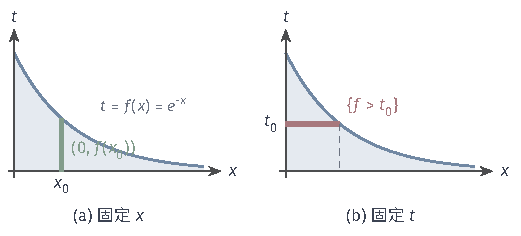
\includegraphics[width=88.149mm]{figures/02-abstract-mathematics/01-metric-and-measure/tikz/c3-layer-cake/figure.pdf}
\caption{层饼公式的两种切法，$f(x)=e^{-x}$，纵轴放大两倍绘制。(a)固定$x_0=0.8$，竖直截面是$(0,f(x_0))$，长度$e^{-0.8}\approx0.449$；(b)固定$t_0=0.4$，水平截面是$\{f>t_0\}=[0,-\ln0.4)\approx[0,0.916)$。两种截面长度分别对$x$和对$t$累计，都得到阴影区域的面积$1$。}
\label{fig:integral-layer-cake}
\end{figure}
